\documentclass{article}
\usepackage{tempora}
\usepackage{hyphenat}
\usepackage{indentfirst}
\usepackage{tabularx}
\usepackage{caption}
\usepackage{graphicx}
\graphicspath{ {./images/} }
\usepackage{float}
\usepackage[english, russian]{babel}
\usepackage{tabularray}
\usepackage{longtable}
\usepackage{color}
\usepackage{booktabs}
\usepackage[table]{xcolor}
\usepackage{mathtools}
\usepackage{hhline}


\begin{document}

    % Название статьи
    \begin{center}
    \Large
    \textbf{}
    \end{center}

    \begin{center}
        Шаблий А.Д.
    \end{center}

    \section*{Аннотация}
    % Цели и задачи
% Краткое описание:
% 1. Методологии исследования
% 2. Результатов
% 3. Актуальность и значимость исследования

% 150-200 слов

Некоторый текст анотации




    \section*{Введение}
    % Какие аналогичные задачи решаются по смежной тематике
Описание актуальных проблем в сфере информационных технологий в целом и области разработки ПО в частности на языке математики и составление математических моделей выполняется для широкого спектра проблем. В работе [] рассматривается решение задачи для организации зависимостей и решения проблемы dependency hell. Организация расписания использования разделяемых ресурсов описывается в работе []. Пример решения задачи об иерархии использования наследования классов приведен в работе []. 

Проанализировав работы [], [] и [] можно сделать вывод, что оптимизировать необходимо не только техническую реализацию актуальных задач, но и стоимость решения как программного продукта. Снижение его стоимости может достигаться разными способами. В настоящей работе рассматривается достижение стоимости за счет оптимизации расходов на его постпродажное обслуживание (ППО).

Анализ показал, что стоимость ППО зависит от объема [], характера [] и сложности организации комплексной работы функционала [], реализованного в ПО. Так, например, дополняющий друг друга функционал может снижать стоимость ППО []. Повышать стоимость ППО могут, например, конкурирующие за разделяемый ресурс единицы функционала [].

% Про плагины
Была выдвинута гипотеза, что снижения стоимости ППО может быть достигнуто путем исключения из решения незаявленного (бесполезного) для заказчика функционала. Такой способ был бы актуален для решений, которые динамически формируют конечный функционал программного комплекса, вносят в него новый функционал и изменяют существующий. Примером таких решений являются плагинные системы [], []. В них интеграционными функциональными единицами являются плагины [], [], [].

% На какие вопросы рассматриваемые ранее задачи ответили
После изучения работ [], [] и [], был сделан вывод, что в решаемой задаче необходимо учесть:
\begin{itemize}
  \item число требований - в них описываются функциональные возможности ПО
  \item число файлов исходного кода - в них на языке программирования реализованы требования
  \item число плагинов - они включают в себя файлыы исходного кода
  \item трассируемость требований на файлы исходного кода
  \item зависимости между файлами исходного кода
  \item распределение файлов исходного кода по плагинам
\end{itemize}

% На какие вопросы рассматриваемые ранее задачи не ответили
Благодаря этим сведениям можно построить метаматическую модель, отвечающую на вопрос, какие требования будут реализованы в поставке. Однако если имеющуюся информацию дополнить сведениями о стоимости сопровождения требований и механизмами формирования результирующей стоимости, тогда может быть решена задача оптимизации внутренней структуры программного решения по критерию минимальной стоимости ППО.


    \section*{Описание модели}
    \subsection*{Постановка задачи}
Основывываясь на вышеизложенном, была предложена следующая формулировка задачи, решение которой предполагается выполнять:

<<Пусть имеется $n$ требований к ПО, которые трассируются на $m$ файлов исходного кода. Файлы распределены по $k$ плагинам. Требуется определить оптимальное распределение файлов по плагинам для минимальной стоимости сопровождения возможных поставок в заявленных $l$ комплектациях. Стоимость сопровождения требования в рамках поставки зависит от состава поставки и может изменяться от наличия или отсутствия реализованных в поставке других требований>>.

\subsection*{Комплектации}
Решение, выполненное в виде комплекса плагинов, может быть поставлено более чем в одной комплектации. В рамках каждой из заявленных комплектаций каждое из возможных требований маркируется либо как \textit{полезное}, либо как \textit{бесполезное}. Поставка должна включать все \textit{полезные} требования. Присвоенные признаки полезности каждому из требований во всех заявленных комплектациях образуют матрицу бинарных отношений $E_{l \times n}$. Элемент $e_{i, j} = 0$ если в рамках $i$-й комплектации $j$-е требование \textit{бесполезно} и $1$ если \textit{полезно}.

\subsection*{Цена постпродажного обслуживания}
Цена постпродажного обслуживания каждого отдельного требования может отличаться в разных поставках. Это происходит из-за того, что по условию задачи наличие других реализованных требований в поставке изменяет цену сопровождения требования и может его как уменьшать, так и увеличивать. Образуется матрица изменения стоимости сопровождения требований $C_{n \times n}$. В ней указывается, на сколько изменится цена сопровождения $i$-го требования, если в поставке будет реализовано $j$-е.

\subsection*{Трассируемость требований к ПО на файлы исходного кода}
Каждое требование трассируется на файлы исходного кода. Для реализации требования в поставке в нее должны быть включены все файлы, которые реализуют данное требование. При этом каждое из требований может быть реализовано в одном или нескольких файлах, а каждый файл может реализовывать одно или несколько требований. Так образуется матрица трассируемости $T_{n \times m}$. Каждый из элементов матрицы имеет значение в диапазоне $[0;1]$. Значение определяет условную долю участия файла в реализации требования. Если $j$-й файл не задействован в реализации $i$-го требования, то значение $t_{i, j} = 0$, иначе $0 < t_{i, j} \le 1$. При этом выполняются условия:
\begin{center}
  $\displaystyle \sum^{m}_{j = 1}t_{1, j} = 1, 
    \sum^{m}_{j = 1}t_{2, j} = 1, \cdots, \sum^{m}_{j = 1}t_{n, j} = 1$
\end{center}

\subsection*{Зависимости между файлами исходного кода}
Файлы исходного кода могут иметь зависимости друг на друга. Без разрешения зависимостей файл не может быть включен в поставку. Т.к. число возможных зависимостей у каждого из файлов не может превышать общее число файлов, зависимости между ними описывает матрица бинарных отношений $D_{m \times m}$. В ней элемент $d_{i, j} = 0$ если у $i$-го файла нет зависимости от $j$-го и равен $1$ если зависимость есть. Файл не зависит сам от себя. Поэтому значения элементов на главной диагонале равны $0$.

\subsection*{Распределение файлов исходного кода по плагинам}
Файлы исходного кода распределены по плагинам. Один файл может быть включен только в один плагин, в то время как один плагин может включать в себя множество файлов. Образуется матрица бинарных отношений $A_{m \times k}$. Элемент $a_{i, j} = 0$ если $i$-й файл не включен в $j$-й плагин и равен $1$ если включен. Кроме того на элементы матрицы $A$ действуют ограничения:
\begin{center}
  $\displaystyle \sum^{k}_{j = 1}a_{1, j} = 1, \sum^{k}_{j = 1}a_{2, j} = 1, \cdots, \sum^{k}_{j = 1}a_{m, j} = 1$
\end{center}
Решение задачи поиска оптимальной декомпозиции заключается в нахождении именно этих коэффициентов.

\subsection*{Целевая функция}
Целевая функция может быть записана как минимизация стоимостей поставок во всех возможных комплектациях:
\begin{center}
  $\displaystyle min \sum^{l}_{i = 1} f_{c}(E_{i})$
\end{center}

где $f_{c}$ - функция стоимости сопровождения комплектации. Алгоритм работы этой функции:

\begin{enumerate}
  \item Определить вектор полезных требований $R_{1 \times n}$. Является входным аргументом функции $f_{c}$.
  \item Вычислить вектор полезных файлов исходного кода:
  \begin{center}
    $F_{1 \times m} = R \cdot T$
  \end{center}
  \item Определить минимально необходимый перечень файлов исходного кода для осуществления поставки в заданной комплектации. Для этого вычислить сумму $F$ и разрешенных зависимостей: 
  \begin{center}
    $\displaystyle \hat{F}_{1 \times m} = F + \sum^{m}_{j = 1}f_{dep}(j)$
  \end{center}
  Описание функции $f_{dep}$ приведено далее.
  \item Определить плагины, которые должны войти в поставку:
  \begin{center}
    $P_{1 \times k} = f_{in}(\hat{F} \cdot A)$
  \end{center}
  \begin{center}
    $\dot{P}_{k \times 1} = P^{T}$
  \end{center}
  \begin{center}
    $
    f_{in} =
    \begin{cases}
      0 & \quad \text{если } x = 0 \\
      1 & \quad \text{если } x > 0
    \end{cases}
    $
  \end{center}
  \item Определить все файлы исходного кода, которые должны войти в поставку:
  \begin{center}
    $\dot{F}_{m \times 1} = A \cdot \dot{P}$
  \end{center}
  \item Определить все реализованные требования в поставке:
  \begin{center}
    $\dot{R}_{n \times 1} = f_{im}(T \cdot \dot{F})$
  \end{center}
  \begin{center}
    $
    f_{im} =
    \begin{cases}
      0 & \quad \text{если } x < 1 \\
      1 & \quad \text{если } x \geq 1
    \end{cases}
    $
  \end{center}
  \item Рассчитать стоимость сопровождения комплектации:
  \begin{center}
    $\dot{R}^{T} \cdot (С \cdot \dot{R})$
  \end{center}
\end{enumerate}

Таким образом целевая функция - это:
  \begin{center}
    $\displaystyle min \sum^{l}_{i = 1} \Bigg[\Bigg[f_{im}\Bigg(T \cdot \bigg(A \cdot \bigg[f_{in}\Big(\big(E_{i} \cdot T + \sum^{m}_{j = 1}f_{dep}(j)\big) \cdot A\Big)\bigg]^{T}\bigg)\Bigg)\Bigg]^{T} \cdot \Bigg[C \cdot~f_{im}\Bigg(T~\cdot~\bigg(A \cdot \bigg[f_{in}\Big(\big(E_{i} \cdot T + \sum^{m}_{j = 1}f_{dep}(j)\big) \cdot A\Big)\bigg]^{T}\bigg)\Bigg)\Bigg]\Bigg]$
  \end{center}

\subsection*{Функция разрешения зависимостей между файлами исходного кода}
Функция разрешения зависимостей между файлами исходного кода $f_{dep}$ позволяет определять перечень зависимостей среди файлов на каждом из слоев зависимостей. Слой зависимости определяет глубину, на которой проводится поиск зависимостей. Так, зависимости $F$ имеют уровень $1$. Их зависимости уровень $2$ и т.д. Заметим, что число слоев не может превышать общее число файлов исходного кода $m$.

Например, пусть задача решается для четырех файлов исходного кода. Ниже приведен пример вектора $F$ и матрицы $D$ для этого случая:
\begin{center}
  $
    F = \begin{pmatrix}
      1 & 0 & 0 & 0 
    \end{pmatrix}
  $
\end{center}
\begin{center}
  $
    D = \begin{pmatrix}
    0 & 1 & 0 & 0 \\
    0 & 0 & 1 & 1 \\
    0 & 0 & 0 & 0 \\
    0 & 0 & 0 & 0 
    \end{pmatrix}
  $
\end{center}
Значения элементов вектора $F$ говорят о том, что полезным является только первое требование. Значения элементов матрицы $D$ говорят, что:
\begin{itemize}
  \item Файл № $1$ имеет зависимость на файл № $2$
  \item Файл № $2$ имеет зависимости на файлы № $3$ и № $4$
  \item Файл № $3$ не имеет зависимостей
  \item Файл № $4$ не имеет зависимостей
\end{itemize}
Тогда зависимости уровня $1$:
\begin{center}
  $
  \begin{pmatrix}
    1 & 0 & 0 & 0 
  \end{pmatrix}
  \cdot
  \begin{pmatrix}
    0 & 1 & 0 & 0 \\
    0 & 0 & 1 & 1 \\
    0 & 0 & 0 & 0 \\
    0 & 0 & 0 & 0 
  \end{pmatrix}
  = 
  \begin{pmatrix}
    0 & 1 & 0 & 0 
  \end{pmatrix}
  $
\end{center}
У полезных файлов $F$ присутствует зависимость только на файл № $2$. Это соответствует заданной матрице $D$. Если полученный вектор умножить заново на матрицу $D$, то будут вычислены файлы для разрешения зависимостей их уровня:
\begin{center}
  $
  \begin{pmatrix}
    0 & 1 & 0 & 0 
  \end{pmatrix}
  \cdot
  \begin{pmatrix}
  0 & 1 & 0 & 0 \\
  0 & 0 & 1 & 1 \\
  0 & 0 & 0 & 0 \\
  0 & 0 & 0 & 0 
  \end{pmatrix}
  = 
  \begin{pmatrix}
    0 & 0 & 1 & 1 
  \end{pmatrix}
  $
\end{center}

Исходя из этого $f_{dep}$ можно записать как рекурсивную функцию:
\begin{center}
  $
  f_{dep}(x) = 
  \begin{cases}
    F \cdot D & \quad \text{если } x = 1 \\
    f_{dep}(x - 1) \cdot D & \quad \text{если } x > 1
  \end{cases}
  $
\end{center}
где $x$ - уровень вложенности зависимостей.

Примечателен тот факт, что значение элемента не важно. Если оно больше $0$, значит элемент активен.


    \section*{Программная реализация}
    Описанная модель реализована на языке программирования Java. Реализация сочетает достоинства применения как парадигмы ООП, так и процедурного программирования. При реализации обособлен выбор типа задействованной коллекции для описания набора вершин и дуг.

% Обозначить, что правильный выбор коллекции - это залог успеха
При проектировании программной реализации было выявлено, что на производительность решения существенное влияние оказывает способ хранения информации о вершинах и дугах. Вариативность способов хранения этой информации зависит от выбранного языка программирования и объема подключаемых библиотек.

% Массивы
Используемый в работах [10], [16], [18] способ хранения информации в массивах является самым простым в реализации. Его использование позволяет наиболее эффективно осуществлять поиск элементов и осуществлять обновление информации о наличествующих в графе вершинах и дугах. Например, как показано в работе [13], изменять значение весовых коэффициентов. Данный способ наиболее эффективно использовать при работе на статическом графе, который не изменяется с течением времени. Использование его в динамически изменяющимся графе приведет к необходимости создания новых экземпляров массивов с последующим заполнением их значений.

% Списки
Для проектирования динамически изменяющегося графа необходимо применять динамические структуры данных. Примером таких динамически изменяющихся структур являются связные списки. В работе [4] рассматривается пример их использования. Однако списки допускают хранение одинаковых элементов, что при проектировании описанной графовой модели недопустимо. Модель не предусматривает наличие уникальных идентификаторов. Вследствие этого было принято решение об использовании множеств уникальных значений (Set).

% Многомерные массивы
Еще одним важным вопросом при проектировании был способ организации связности данных между собой. Необходимо хранить информацию, какие вершины связаны, какая является начальной, а какая конечной. В работе [2] приводится пример использования многомерных массивов. Однако, как описано ранее, данный подход эффективен при неизменяемом числе связей между компонентами графа. Например, если у каждой вершины зафиксировано число дуг, а в процессе преобразований графа моделью изменяется информация о том, в какие именно дуги соединяют вершину с другими вершинами графа. При проектировании модели, в которой число дуг у вершины графа может изменяться, могут создаваться новые вершины и дуги, удаляться ранее созданные, эффективным представляется использование так же динамических структур данных. При проектировании этого функционала было принято решение об использовании множеств уникальных значений (Set).

Выбранная структура данных может быть реализована по-разному. Выбор реализации влияет на время работы программной реализации модели. С целью проведения экспериментов и получения информации о зависимости времени работы программы от числа элементов графа в реализации предусмотрены два модуля:
\begin{enumerate}
    \item модуль определения реализации коллекции Set;
    \item модуль генерации исходных данных.
\end{enumerate}

Модуль определения реализации коллекции Set выполнен с целью определения временных характеристик работы программной реализации модели при условии использования различных реализаций этой коллекции. Благодаря использованию этого модуля достигается возможность задания конкретной реализации с последующим ее внедрением в исходный код программной реализации модели. Модуль позволяет внедрять как стандартные реализации коллекции Set, так и реализации, хранящиеся в подключаемых библиотеках или самостоятельно реализованные пользователем.

Модуль генерации исходных данных выполнен с целью сокращения времени на подготовку матрицы трассируемости требований на файлы исходного кода и матрицы зависимостей между файлами исходного кода. В качестве входных данных модуль принимает четыре параметра:
\begin{enumerate}
    \item Fc - число файлов исходного кода;
    \item Rc - число требований к ПО;
    \item Mfc - максимальное число зависимостей у файла исходного кода;
    \item Mfr - максимальное число реализуемых требований в одном файле;
\end{enumerate}

    \section*{Эксперименты и обсуждение}
    % Дать трактовку данных, полученных в результате исследования
% Повторно проанализировать сходства и различия в подходах, а так же общее восприятие исследования
% Провести сравнение результатов с достижениями других исследователей в данной области

% 2 ссылки на литературу

В целях проверки работоспособности программной реализации описанной модели проводился ряд экспериментов. В качестве входных данных использовались значения числа элементов графа в различных числовых диапазонах.

В таблицах \ref{tab:hashset}-\ref{tab:treeset} приведены сведения о среднем времени выполнения операций в экспериментах по преобразованию $G$ в $G'$, которые были выполнены по 1000 раз каждый при заданных параметрах генератора исходных данных для следующих реализаций коллекции Set:
\begin{enumerate}
    \item HashSet - таблица \ref{tab:hashset};
    \item LinkedHashSet - таблица \ref{tab:linkedhashset};
    \item TreeSet - таблица \ref{tab:treeset}.
\end{enumerate}

На рисунке \ref{fig:bar} приводится графическая интерпретация результатов экспериментов.

\begin{longtable}{|c|c|c|c|c|c|}
    \caption{Результаты работы программной реализации с применением HashSet}
    \label{tab:hashset}\\   
    \hline
    \bfseries{№} & \bfseries{Fc} & \bfseries{Rc} & \bfseries{Mfc} & \bfseries{Mfr} & \bfseries{Средне время, мс} \\
    \hline
    \endfirsthead
    \hline
    \bfseries{№} & \bfseries{Fc} & \bfseries{Rc} & \bfseries{Mfc} & \bfseries{Mfr} & \bfseries{Средне время} \\
    \hline
    \endhead
    \hline
    1 & 100 & 100 & 30 & 30 & 42 \\
    \hline
    2 & 100 & 100 & 30 & 50 & 52 \\
    \hline
    3 & 100 & 100 & 50 & 30 & 60 \\
    \hline
    4 & 100 & 100 & 50 & 50 & 41 \\
    \hline
    5 & 100 & 1000 & 30 & 300 & 57 \\
    \hline
    6 & 100 & 1000 & 30 & 500 & 77 \\
    \hline
    7 & 100 & 1000 & 50 & 300 & 63 \\
    \hline
    8 & 100 & 1000 & 50 & 500 & 65 \\
    \hline
    9 & 1000 & 100 & 300 & 30 & 7830 \\
    \hline
    10 & 1000 & 100 & 300 & 50 & 7402 \\
    \hline
    11 & 1000 & 100 & 500 & 30 & 8364 \\
    \hline
    12 & 1000 & 100 & 500 & 50 & 8163 \\
    \hline
    13 & 1000 & 1000 & 300 & 300 & 6932 \\
    \hline
    14 & 1000 & 1000 & 300 & 500 & 6807 \\
    \hline
    15 & 1000 & 1000 & 500 & 300 & 8191 \\
    \hline
    16 & 1000 & 1000 & 500 & 500 & 8496 \\
    \hline
\end{longtable}

\begin{longtable}{|c|c|c|c|c|c|}
    \caption{Результаты работы программной реализации с применением LinkedHashSet}
    \label{tab:linkedhashset}\\
    \hline
    \bfseries{№} & \bfseries{Fc} & \bfseries{Rc} & \bfseries{Mfc} & \bfseries{Mfr} & \bfseries{Средне время} \\
    \hline
    \endfirsthead
    \hline
    \bfseries{№} & \bfseries{Fc} & \bfseries{Rc} & \bfseries{Mfc} & \bfseries{Mfr} & \bfseries{Средне время} \\
    \hline
    \endhead
    \hline
    1 & 100 & 100 & 30 & 30 & 37 \\
    \hline
    2 & 100 & 100 & 30 & 50 & 52 \\
    \hline
    3 & 100 & 100 & 50 & 30 & 40 \\
    \hline
    4 & 100 & 100 & 50 & 50 & 29 \\
    \hline
    5 & 100 & 1000 & 30 & 300 & 88 \\
    \hline
    6 & 100 & 1000 & 30 & 500 & 48 \\
    \hline
    7 & 100 & 1000 & 50 & 300 & 52 \\
    \hline
    8 & 100 & 1000 & 50 & 500 & 71 \\
    \hline
    9 & 1000 & 100 & 300 & 30 & 4061 \\
    \hline
    10 & 1000 & 100 & 300 & 50 & 2894 \\
    \hline
    11 & 1000 & 100 & 500 & 30 & 3065 \\
    \hline
    12 & 1000 & 100 & 500 & 50 & 3083 \\
    \hline
    13 & 1000 & 1000 & 300 & 300 & 2755 \\
    \hline
    14 & 1000 & 1000 & 300 & 500 & 2892 \\
    \hline
    15 & 1000 & 1000 & 500 & 300 & 3017 \\
    \hline
    16 & 1000 & 1000 & 500 & 500 & 3415 \\
    \hline
\end{longtable}

\begin{longtable}{|c|c|c|c|c|c|}
    \caption{Результаты работы программной реализации с применением TreeSet}
    \label{tab:treeset}\\
    \hline
    \bfseries{№} & \bfseries{Fc} & \bfseries{Rc} & \bfseries{Mfc} & \bfseries{Mfr} & \bfseries{Средне время} \\
    \hline
    \endfirsthead
    \hline
    \bfseries{№} & \bfseries{Fc} & \bfseries{Rc} & \bfseries{Mfc} & \bfseries{Mfr} & \bfseries{Средне время} \\
    \hline
    \endhead
    \hline
    1 & 100 & 100 & 30 & 30 & 65 \\
    \hline
    2 & 100 & 100 & 30 & 50 & 71 \\
    \hline
    3 & 100 & 100 & 50 & 30 & 70 \\
    \hline
    4 & 100 & 100 & 50 & 50 & 52 \\
    \hline
    5 & 100 & 1000 & 30 & 300 & 51 \\
    \hline
    6 & 100 & 1000 & 30 & 500 & 58 \\
    \hline
    7 & 100 & 1000 & 50 & 300 & 78 \\
    \hline
    8 & 100 & 1000 & 50 & 500 & 119 \\
    \hline
    9 & 1000 & 100 & 300 & 30 & 8083 \\
    \hline
    10 & 1000 & 100 & 300 & 50 & 6264 \\
    \hline
    11 & 1000 & 100 & 500 & 30 & 7509 \\
    \hline
    12 & 1000 & 100 & 500 & 50 & 7562 \\
    \hline
    13 & 1000 & 1000 & 300 & 300 & 6640 \\
    \hline
    14 & 1000 & 1000 & 300 & 500 & 6911 \\
    \hline
    15 & 1000 & 1000 & 500 & 300 & 7982 \\
    \hline
    16 & 1000 & 1000 & 500 & 500 & 7705 \\
    \hline
\end{longtable}

\begin{figure}[H]
    \centering
    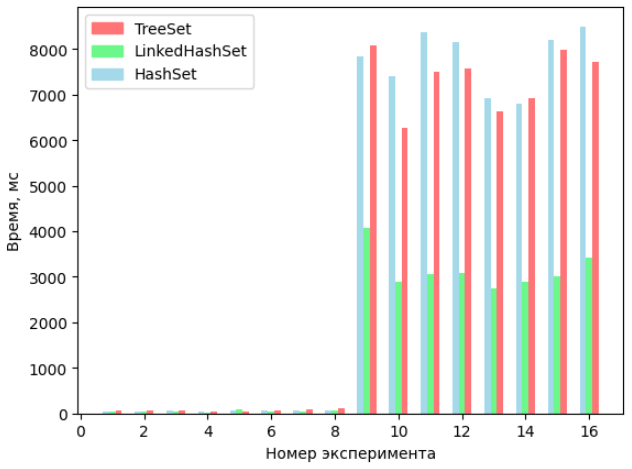
\includegraphics[width=1\textwidth]{bar}
    \caption{Графическая интерпретация результатов экспериментов}
    \label{fig:bar}
\end{figure}

Результаты экспериментов показывают, что резкое увеличение времени выполнения преобразования графа происходит при увеличении числа файлов исходного кода, а значительное увеличение числа требований к ПО к такому эффекту не приводит.

В среднем наибольшее время требуется при работе с реализацией HashSet - 8496 мс. Наименьшее время требуется при работе с LinkedHashSet. При использовании этой реализации коллекции Set наибольшее среднее время составляет 4061 мс, в то время как для TreeSet максимальное значение среднего времени достигает 8083 мс при наибольшем количестве файлов исходного кода.

    \section*{Заключение}
    % Формулируются выводы сделанные на основе проведенного исследования
% Удалось ли реализовать поставленные задачи и достигнуть целей
% Подчеркнуть вклад исследования в развитие научной области, какие перспективы открывают полученные данные для научного сообщества
% Кто и каким образом сможет применить новые знания на практике в будущем
% Какие моменты в исследовании нуждаются в дополнительной проработке или углабленно анализе

% 2 ссылки на литературу

В статье предложена модель, отображающая трассируемость требований к ПО на файлы исходного кода и позволяющая разрешать циклические зависимости между файлами исходного кода. Используя ее можно получать информацию о степени связности файлов исходного кода друг с другом, на какую долю функционала оказывается влияние при внесении изменений в файлы исходного кода. Данные сведения могут быть полезны при оценке необходимого объема выполнения верификационных процедур после внесения изменений в один или несколько файлов исходного кода.

В дальнейших исследованиях предполагается применение результатов работы сформированной модели для решения задачи оптимальной декомпозиции на выполненной как модуль плагинной системы программной реализации инструментального средства конфигурирования. Предполгается использовать результаты работы модели для распределения файлов исходного кода по плагинам с целью максимизации числа возможных комплектаций.

    \section*{Литература}
    \begin{enumerate}
    \item А.Н. Вигура, анализ и тестирование программ на основе алгебраической модели, Информационные технологии, Вестник Нижегородского университета им. Н.И. Лобачевского, 2011, No 5 (1), с. 185–190;
    \item А.М. Шульженко, автоматическое определение циклов ParDo в программе, Естественные науки, известия ВУЗов. северо-кавказский регион, ISSN 0321-3005, с. 77-87;
    \item B. П. Корячко, д-р техн. наук проф., C. В. Скворцов, канд. техн. наук доц., Иерархическая модель глобальной оптимизации у параллельных объектных программ, электронный журнал "Инженерное образование", 2006; 
    \item Кошелев В.К., Игнатьев В.Н., Борзилов А.И. Инфраструктура статического анализа программ на языке C\#. Труды ИСП РАН, том 28, вып. 1, 2016 г., с. 21-40;
    \item А. А. Чертков, Я. Н. Каск, Л. Б. Очина, Маршрутизация потоковой сети на основе модификации алгоритма Беллмана - Форда, ФГБОУ ВО «ГУМРФ имени адмирала С. О. Макарова», Санкт-Петербург, Российская Федерация, 2022г, топ 14 № 4, с 615-627;
    \item В. В. Сахаров, А. А. Чертков, Л. Б. Очина, Маршрутизация сетей с отрицательными весами звеньев в пакете оптимизации MATLAB ФГБОУ ВО «ГУМРФ имени адмирала С. О. Макарова», Санкт-Петербург, Российская Федерация, 2019г, том 11 № 2, с 230-242;
    \item К.В. Недоводеев, Метод генерации графов потоков данных, используемых при автоматическом синтезе параллельных программ для неоднородных многоядерных процессов, Научно-технические ведомости СПбГПУ 3' 20122 Информатика. Телекоммуникации. Управление, с 47-52;
    \item Ю. И. Евсеева, А. C. Бождай, Метод синтеза адаптивных программных компонентов виртуальной образовательной среды, Известия высших учебных заведений. Поволжский регион, DOI 10.21685/2072-3059-2016-3-8, с 84-92;
    \item О.А. Четверина, Методы коррекции профильной информации в процессе компиляции, Труды ИСП РАН, том 27, вып. 6, 2015 г. с 49-65;
    \item О.Б. Штейнберг, Минимизация количества временных массивов в задаче разбиения циклов, ISSN 0321-3005 известия ВУЗов, Северо-Кавказский регион, естественные науки, 2011. № 5, с 31-35;
    % \item Н. В. Заборовский, А. Г. Тормасов, докт. физ.‑мат. наук, Моделирование многопоточного исполнения программы и метод статического анализа кода на предмет состояний гонки, 
    \item Тарков М. С., Об эффективности построения гамильтоновых циклов в графах распределенных вычислительных систем рекуррентными нейронными сетями, Информационные технологии в управлении, Институт физики полупроводников им. А.В. Ржанова СО РАН, Новосибирск, Управление большими системами. Выпуск 43, 2013, с 157-171;
    \item С.В. Огородов, Обоснование линейноупорядоченного представления графовых моделей программ, Институт «Кибернетический центр» ТПУ, Известия Томского политехнического университета. 2008. Т. 312. № 5, с 85-89;
    \item Фролов А. С., канд. техн. наук Семенов А. С, Обзор проблемно-ориентированных языков программирования для параллельного анализа статических графов, Computational nanotechnology 1-2017, ISSN 2313-223X, 27-32;
    \item Е. П. Емельченков, В. И. Мунерман, Д. В. Мунерман, Т. А. Самойлова, Один метод построения циклов в графе, Современные информационные технологии и ИТ-образование. 2021. Т. 17, № 4. С. 814-823 
    \item А.А. Каленкова, Оптимизация потоков работ по времени выполнения, основанная на удалении избыточных потоков управления, ТРУДЫ МФТИ. — 2009. — Том 1, № 2, 160-174;
    \item А.П. Баглий, Н.М. Кривошеев, Б.Я. Штейнберг, О.Б. Штейнберг, Преобразования программ в Оптимизирующей распараллеливающей системе для распараллеливания на распределенную память, Инженерный вестник Дона, №12 (2022), ivdon.ru/ru/magazine/archive/n12y20225/8089;
    \item О.Б. Штейнберг, И.А. Ивлев, Применение преобразования циклов "Retiming" с целью уменьшения количества используемых регистров, Южный федеральный университет, г. Ростов-на-Дону, Россия, ISSN 0321-2653 известия ВУЗов. Северо-Кавказский регион. Технические науки. 2017. № 3, с 76-80;
    \item А. Ю. Попов, Применение вычислительных систем смногими потоками команд и одним потоком данных для решения задач оптимизации, ISSN 0236-3933. Вестник МГТУ им. Н.Э. Баумана. Сер. "Приборостроение", 2012, с 146-154; 
    \item Карпов Ю.Л., Волкова И.А., Вылиток А.А., Карпов Л.Е., Сметанин Ю.Г. Проектирование интерфейсов классов графовой модели нейронной сети. Труды ИСП РАН, том 31, вып. 4, 2019 г., стр. 97-112.
\end{enumerate}

\end{document}